\documentclass[11pt]{article}
\usepackage[portuges]{babel}%Babel -- irá activar automaticamente as regras apropriadas de hifenização para a língua todo o
                                   %-- o texto gerado é automaticamente traduzido para Português.
                                   %  Por exemplo, “chapter” irá passar a “capítulo”, “table of contents” a “conteúdo”.
                                   % portuges -- específica para o Português.
\usepackage[utf8]{inputenc} % define o encoding usado texto fonte (input)--usual "utf8" ou "latin1
\usepackage[T1]{fontenc}
\usepackage{graphicx}
%\usepackage{layout}

%used to fix header space
\usepackage[headheight=0pt,headsep=0pt]{geometry}
\addtolength{\topmargin}{-40pt}
\addtolength{\textheight}{120pt}

\usepackage{tabularx}

\title{Laboratórios de Informática III \\
       \textbf{Trabalho Prático C}\\ Relatório de Desenvolvimento
       } %Titulo do documento
\author{Pedro Costa\\ (a85700) \and Miguel Caravalho\\ (A84518)
         \and Maria João Moreira\\ (A89540)
       } %autores do documento
\date{06-04-2020} %data


\begin{document}
\begin{titlepage}
    
\includegraphics[width=\columnwidth]{images/capa.pdf}
\end{titlepage}
\newpage

\newpage
\tableofcontents %insere o índice

\newpage
\section{Introdução}
Tal como é dito no enunciado deste projeto, o desenvolvimento desta aplicação tem por objetivo consolidar, com ênfase na parte prática, os conhecimentos adquiridos noutras UCs (nomeadamente \textit{Algoritmos e Complexidade}) e, ainda, introduzir \textbf{novos princípios de programação} aplicáveis à programação em média-larga escala.

Tal como em vários projetos de média-larga escala, no desenvolvimento desta aplicação lidamos com grandes volumes de dados e foi imperativo ter em consideração o uso de estruturas adequadas para armazenar os ditos dados e ser capazes de os consultar de forma eficiente.

\section{Módulos e funcionalidades correspondentes}

\subsection{Componentes principais do SGV - Visão superficial}
O módulo principal da nossa aplicação, o \textbf{SGV} é composto pelas seguintes componentes, tal como foi pedido.

\begin{itemize}
    \item \textbf{Catálogo de Produtos}: Módulo de dados onde se guarda todos os códigos de produtos válidos lidos.
    \item \textbf{Catálogo de Clientes}: Igual ao Catálogo de Produtos mas guarda códigos de clientes.
    \item \textbf{Faturação}: Módulo de dados que relaciona produtos com informação relativa às suas vendas (quantidades vendidas e lucros).
    \item \textbf{Filial}: Módulo de dados que relaciona clientes com os produtos que compram para \textbf{uma} dada filial (saber quanto comprou e quanto gastou em todos os produtos que obteve).
\end{itemize}

\vspace{1cm}
\begin{figure}[h]
    \centering
    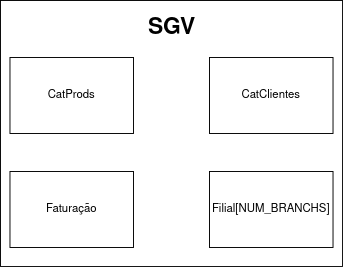
\includegraphics[width=\textwidth,height=5cm]{images/sgv.png}
    \caption{Componentes do SGV}
\end{figure}

\newpage
\subsubsection{Catálogo - A estrutura de dados mais eficiente para a nossa aplicação}
Ainda que não seja uma das estruturas principais do SGV, o módulo de dados \textbf{Catalog} é, sem sombra de dúvidas, o ponto central do nosso projeto. Todas as componentes do SGV foram definidas à custa deste módulo uma vez que permite acessos extremamente rápidos aos códigos que contém.

Este módulo é composto por um array de GTree* em que cada \textit{tree} corresponde a todas as chaves começadas por um conjunto de letras (\textit{ie.} "A", "ZD", "FRW", etc...).

Esta estrutura assemelha-se muito a um dicionário, catalogando as chaves que contém de acordo com a sua nomenclatura. O esquema abaixo explica melhor como está desenhado este módulo.

\textbf{Nota}: Todos os valores inseridos nas trees tem chave correspondente à parte numérica do código introduzido.

\vspace{1cm}
\begin{figure}[h]
    \centering
    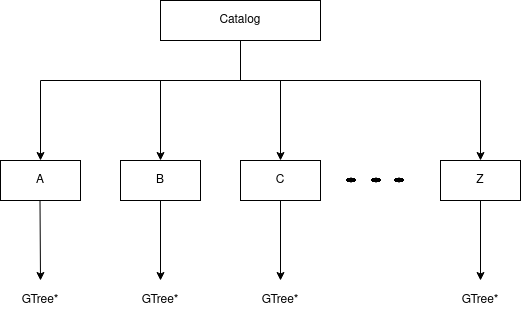
\includegraphics[width=\textwidth,height=5cm]{images/catalog.png}
    \caption{Catalog}
\end{figure}

Esta estrutura tem uma complexidade de $O(1 + \log_2{}n)$, em que \textit{n} corresponde ao maior tamanho possível de cada tree. A tabela seguinte mostra uma análise do valor de \textit{n} para o caso dos clientes e produtos.

\vspace{1cm}
\begin{tabularx}{\textwidth} {
  | >{\centering\arraybackslash}X
  | >{\centering\arraybackslash}X
  | >{\centering\arraybackslash}X
  | >{\centering\arraybackslash}X
  | >{\centering\arraybackslash}X | }
    \hline
    Tipo & LL & UL & n & Nº max acessos \\
    \hline
    Produto  & 1000  & 9000 & 8000 & $1+\log_2{}8000 = 14$ \\
    \hline
    Cliente & 1000 & 5000 & 4000 & $1+\log_2{}4000 = 13$ \\
    \hline
\end{tabularx}

\vspace{1cm}
\textbf{Legenda}: LL = Lower limit; UL = Upper limit

\newpage
\subsubsection{Catálogo de Produtos/Clientes}
Ambos estes módulos são compostos unicamente por um catálogo cujas chaves correspondem à parte númerica código do cliente ou produto em causa. Em ambas as situações, o campo value corresponde à string completa do código.

\subsubsection{Faturação}
A faturação é, como indicado anteriormente, também composta unicamente por um Catalog. Nesse, para cada produto, guarda-se a \textit{struct} indicada abaixo:

\begin{verbatim}
struct productInfo{
    /* Código do produto */
    char* product;
    /* Vendas distribuídas por tipo, filial e mês */
    int sales[2][NUM_BRANCHES][NUM_MESES];
    /* Lucros distribuídos por tipo, filial e mês */
    float profit[2][NUM_BRANCHES][NUM_MESES];
    /* Total de vendas por tipo (útil mas desnecessário) */
    int total_sales[2];
    /* Total de lucro por tipo (útil mas desnecessário) */
    int total_profit[2];
};
\end{verbatim}

\subsubsection{Filial}
Este módulo é também implementado com base num catálogo. Para cada cliente guarda-se uma \textbf{GHashTable*} que armazena a seguinte \textit{struct}:

\begin{verbatim}
struct customerbought{
    /* Código do produto comprado */
    char* product;
    /* Número de compras por tipo ao longo dos meses */
    int n_compras[2][NUM_MESES];
    /* Lucro por tipo ao longo dos meses */
    float total_gasto[2][NUM_MESES];
};
\end{verbatim}

\textbf{Nota}: Apenas este módulo tem uma complexidade ligeiramente mais elevada que os anteriores uma vez que para se obter um valor é necessário fazer uma procura no catálogo e, de seguida, uma procura na \textit{tree} que se obtém.

\newpage
\subsection{Outros módulos desenvolvidos por necessidade/utilidade}
\subsubsection{Parser}
Este módulo tem unicamente o objetivo de fazer parse. Isto implica as seguintes duas funcionalidades:
\begin{itemize}
    \item \textbf{Validação}: Disponibiliza funções capazes de validar códigos de produtos e de clientes. Útil no parse efetuado no controller e dentro do próprio carregamento.
    \item \textbf{Carregamento de dados}: Disponibiliza as funções \textbf{loadCatalog} e \textbf{loadVendas} para carregar catálogos e vendas, respetivamente, a partir de caminhos para os ficheiros a ler.
\end{itemize}

\subsubsection{Config}
Este módulo contém várias funções úteis em mais do que um módulo desenvolvido. Assim evitamos duplicação desnecessária de código.

\subsubsection{Navegador}
Módulo de dados utilizado para navegar grandes quantidades de informação. A sua implementação extremamente simples baseia-se inteiramente em ter um inteiro que marca o sítio de onde se deve a começar a imprimir duma dada lista de strings e em saber que quantidade é que se deve imprimir de cada vez. Consoante o utilizador pede basta subtrair/somar ao ponto de partida o tamanho que imprimos de cada vez.

\subsubsection{Pair}
Tal como o nome indica, esta API define apenas um par. É uma estrutura extremamente útil uma vez que várias vezes nos encontramos numa situação em que queríamos retornar mais do que um valor (com tipos diferentes) sem estar a devolver um \textit{void*} ou aumentar desnecessariamente o número de argumentos.

\subsubsection{PQueue}
Este módulo foi desenvolvido a partir do ficheiro que se encontra na pasta \textit{libs}. Utilizámo-lo nas queries 10, 11 e 12 pois queríamos devolver algo com base numa certa prioridade. Pareceu-nos apenas natural utilizar uma \textit{priority queue} para tal efeito. Fizemos algumas trocas ao original com base em pormenores que nos facilitariam a vida tais como:
\begin{itemize}
    \item Organizar as entradas em key value. Permite-nos utilizar funções de comparação mais simples que não precisam de conhecer o value na íntegra.
    \item Permitir o fornecimento de funções de free das keys e dos values para se limpar automaticamente toda a memória alocada ao fazer destroy e ao fazer dequeue.
    \item Queríamos ainda ter implementado a possibilidade de fazer resize caso se ultrapasse a capacidade máxima. Não foi implementada esta feature.
\end{itemize}

\subsubsection{Sale}
Este módulo define apenas o que é uma venda disponibilizando na sua API funções de inicialização e \textit{gets} para se obter os respetivos valores armazenados.

\subsubsection{Stats}
Ainda que este módulo seja uma componente do SGV, não é essencial para o seu funcionamento pelo que se trata dum móduloe extra. O \textit{Stats} surgiu para satisfazer uma necessidade extremamente simples. Cronometrar qualquer coisa que quisessemos. O código para cronometrar uma função ainda implica algumas linhas pelo que iríamos poluir muito a nossa base de código para fazer \textit{profiling} em condições. Assim, definimos uma maneira simples para efetuar esta tarefa. Basta adicionar à função \textit{init} os nomes do que queremos cronometar e, quando desejarmos, chamar as seguintes funções.

\begin{verbatim}
/* Starts the timer for the given key */
void start_timing(Stats s, const char* key);

/* Agreggates the time into a given key */
void agreggate_timing(Stats s, const char* key);

/* Finishes timing and writes the result to the file associated with a key */
void finish_timing(Stats s, const char* key);
\end{verbatim}

A função \textit{agreggate\_timing} permite cronometrar funções pelas quais passamos mais duma vez, agregando os novos valores a cada utilização.

\subsubsection{Encapsulamento}
Tal como pedido, garantimos que todos os nossos módulos (à exceção do Stats) têm implementações privadas que nunca permitem que qualquer utilizador consiga alterar o SGV duma maneira não desejável. Para esse efeito não abordamos pela abordagem OO mas sim por criar API's mais extensas que permitem ao utilizador interessado (neste caso, o próprio grupo) obter qualquer informação necessária através do SGV.

\newpage
\section{Arquitetura da aplicação}
Foi sugerido que adotássemos uma arquitetura MVC para unir as diversas componentes da nossa aplicação final e, sendo assim, foi exatamente isso que fizemos. No entanto, devido ao que foi explicado na secção \textit{Encapsulamento} temos um pormenor diferente do que seria uma implementação típica de MVC. No nosso caso, é o próprio SGV que manipula os dados internamente para responder às várias queries. O esquema abaixo demonstra bem as interações no nosso projeto.

\vspace{1cm}
\begin{figure}[h]
    \centering
    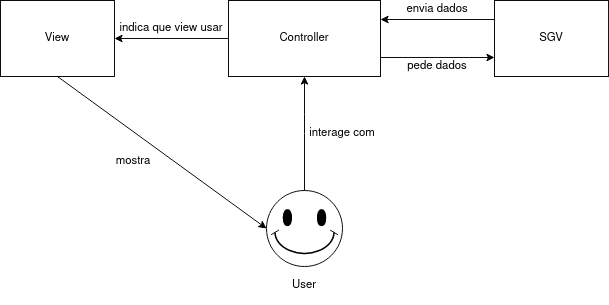
\includegraphics[width=\textwidth,height=10cm]{images/mvc.png}
    \caption{\textbf{Design pattern - MVC}}
\end{figure}

\newpage
\section{Otimizações e profiling}
Tal como referido anteriormente, todo o nosso projeto assenta no módulo de dados \textbf{Catálogo}. Assim, é apenas natural que a maneira mais eficaz de otimizar todo o programa passe por otimizar esse módulo. Assim, oferecemos uma implementação extra do projeto que utiliza um catálogo extremamente mais eficiente mas que consome muita mais memória. Esta implementação encontra-se numa pasta que apelidamos por \textbf{Performance\_Mode} e é um fork do projeto original numa fase em que já se conseguia dar resposta a todas as queries.

A figura abaixo ajuda a compreender a diferença para o \textbf{Catálogo} do projeto principal enviado.

\textbf{Nota}: Esta estrutura tem, literalmente, acessos constantes a cada valor (O(1)).

\vspace{1cm}
\begin{figure}[h]
    \centering
    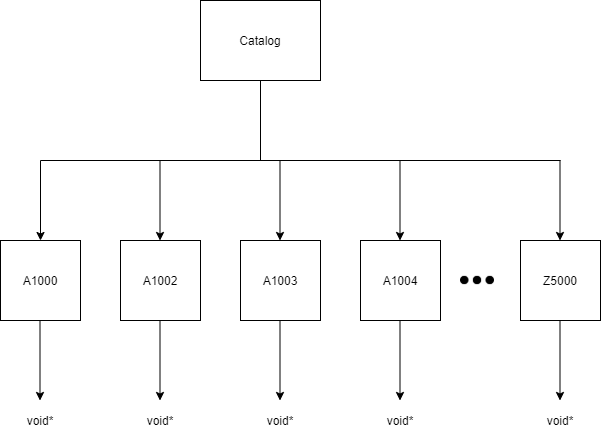
\includegraphics[width=\textwidth,height=5cm]{images/catalogPerformance.png}
    \caption{Optimized catalog}
\end{figure}

Vamos agora comparar exaustivamente todos os tempos medidos (\textbf{Nota}: todos os tempos apresentados são \textit{elapsed times}).

\textbf{Legenda}: TP = Trabalho prático principal; PM = Performance Mode; XM = Ficheiros Vendas\_XM.txt

\vspace{1cm}
\begin{tabularx}{\textwidth} {
  | >{\centering\arraybackslash}X
  | >{\centering\arraybackslash}X
  | >{\centering\arraybackslash}X
  | >{\centering\arraybackslash}X
  | >{\centering\arraybackslash}X
  | >{\centering\arraybackslash}X
  | >{\centering\arraybackslash}X | }
    \hline
    Parsing & TP\_1M & PM\_1M & TP\_3M & PM\_3M & TP\_5M & PM\_5M \\
    \hline
    billProduct & 0.417208 & 0.263402 & 1.518986 & 0.874880 & 2.396639 & 1.532954 \\
    \hline
    cBought & 0.858921 & 0.626829 & 3.200031 & 2.151543 & 4.974849 & 3.681399 \\
    \hline
    loadCC & 0.042927 & 0.012049 & 0.024715 & 0.012149 & 0.023263 & 0.012020 \\
    \hline
    loadCP & 0.137195 & 0.068430 & 1.54743 & 0.068709 & 0.134901 & 0.068051 \\
    \hline
    loadVendas & 3.577178 & 2.003663 & 12.628885 & 6.365291 & 19.606948 & 10.791212 \\
    \hline
    catExists & 1.384713 & 0.193839 & 4.765775 & 0.570989 & 7.393718 & 0.985675 \\
    \hline
    words & 0.297074 & 297820 & 0.993529 & 0.870838 & 1.521031 & 1.469308 \\
    \hline
    totalLoad & 3.75 & 1.95 & 11.77 & 5.63 & 17.92 & 9.46 \\
    \hline
\end{tabularx}

\vspace{1cm}
O que se vê de interessante na tabela acima? Principalmente 3 coisas.
\begin{itemize}
    \item Devido a cronometrar funções que são chamadas uma vez por linha das vendas nota-se uma inflação de cerca de 10\% no tempo registado pelo \textit{loadVendas} em comparação com o \textit{totalLoad} quando estes, em teoria, seriam equivalentes.
    \item O grande peso do carregamento centra-se em verificar que os códigos de produto/cliente existem nos catálogos. Em média, com a otimização feita no \textbf{Performance\_Mode} regista-se um aumento entre 7-10 vezes no tempo dessa ação.
    \item A otimização feita no \textbf{Performance\_Mode} regista praticamente metade do tempo total de carregamento em relação ao projeto principal. Uma diferença abismal sem dúvida.
\end{itemize}

\vspace{1cm}
\begin{tabularx}{\textwidth} {
  | >{\centering\arraybackslash}X
  | >{\centering\arraybackslash}X
  | >{\centering\arraybackslash}X
  | >{\centering\arraybackslash}X
  | >{\centering\arraybackslash}X
  | >{\centering\arraybackslash}X
  | >{\centering\arraybackslash}X | }
    \hline
    Queries & TP\_1M & PM\_1M & TP\_3M & PM\_3M & TP\_5M & PM\_5M \\
    \hline
    query2 & 0.002735 & 0.001739 & 0.002209 & 0.001665 & 0.002723 & 0.001681 \\
    \hline
    query3 & 0.000023 & 0.000001 & 0.000005 & 0.000001 & 0.000012 & 0.000001 \\
    \hline
    query4 & 0.202662 & 0.193588 & 0.198692 & 0.199581 & 0.256908 & 0.203211 \\
    \hline
    query5 & 0.006563 & 0.004580 & 0.015275 & 0.004275 & 0.007031 & 0.004717 \\
    \hline
    query6 & 0.065913 & 0.043696 & 0.076181 & 0.039667 & 0.066692 & 0.043802 \\
    \hline
    query7 & 0.000016 & 0.000008 & 0.000038 & 0.000021 & 0.000068 & 0.000034 \\
    \hline
    query8 & 0.345657 & 0.132062 & 0.108621 & 0.131767 & 0.385788 & 0.126734 \\
    \hline
    query9 & 0.006245 & 0.003522 & 0.004330 & 0.003924 & 0.007911 & 0.004902 \\
    \hline
    query10 & 0.00003 & 0.000013 & 0.000113 & 0.000026 & 0.000074 & 0.000035 \\
    \hline
    query11 & 0.480123 & 0.455098 & 1.279723 & 1.170635 & 1.914258 & 1.914663 \\
    \hline
    query12 & 0.000155 & 0.000046 & 0.000155 & 0.000083 & 0.00056 & 0.000140 \\
    \hline
\end{tabularx}

\vspace{1cm}
O que se vê de interessante na tabela acima? E qual a diferença principal que se nota em comparação com a tabela de parsing?
\begin{itemize}
    \item Nesta tabela acontece uma de duas coisas quando comparamos os tempos entre os dois modos diferentes. Ou são iguais, ou o \textbf{Performance\_Mode} é praticamente 2 vezes mais rápido. O primeiro caso deve-se ao facto de a maior parte das queries serem travessias, pelo que não faz diferença o tempo de acesso a cada campo. O segundo caso deve-se ao facto de o acesso à memória ser constante no \textbf{Performance\_Mode}.
    \item A principal com a tabela de parsing é exatamente o que foi dito acima. Os tempos aqui são extremamente parecidos uma vez que não estamos a lidar tanto com acessos à memória, tirando menos proveito da otimização feita.
\end{itemize}

\newpage
\section{Utilização do programa e melhorias a fazer}
A aplicação que desenvolvemos oferece também ao utilizador três flags extremamente úteis para uso continuado.
\begin{itemize}
    \item \textbf{---timing-mode}: Tal como o nome indica, esta flag ativa o timing mode, gravando nos ficheiros correspondentes os tempos obtidos ao longo do programa. (\textbf{Nota}: Tem obrigatoriamente de ser a primeira flag.)
    \item \textbf{---save-queries}: Esta flag permite que todas as queries, além de serem demonstradas na UI ao utilizador, sejam ainda gravadas em ficheiros de texto. Extremamente útil para comparação de resultados.
    \item \textbf{---default-load}: Esta, a nossa favorita, permite pré-carregar o programa sem ter de especificar um a um os ficheiros a serem utilizados.
    \item \textbf{---config=configfile}: Uma opção extremamente prática que permite fornecer alguns dados ao programa através de um ficheiro com configurações. Caso não seja incluída o programa assume um conjunto de predefinições.
\end{itemize}

\textbf{A nível de melhorias do nosso projeto} achamos que não há muito a fazer. Possivelmente melhorar a interface gráfica e adicionar features ao navegador seriam um bom ponto de partida (ex: 2n para andar 2 páginas).

\section{Testes realizados}
Ao longo do desenvolvimento do projeto testamos unitariamente cada módulo separadamente de maneira a garantir que sempre que adicionamos mais código à nossa base, caso houvesse algum erro, este encontrar-se-ia no código adicionado mais recentemente. Assim conseguimos potencialmente nunca ter de fazer uma grande regressão. Numa fase mais avançada, cruzamos os nossos dados com os oferecidos no ficheiro \textbf{"Resultados para comparação"}.

\vspace{1cm}
Ao longo do seu desenvolvimento, todo o código desenvolvido foi testado na ferramenta \textbf{valgrind} para garantir que não existem quaisquer leaks de memória ou acessos ilegais à mesma.

\vspace{1cm}
\begin{figure}[h]
    \centering
    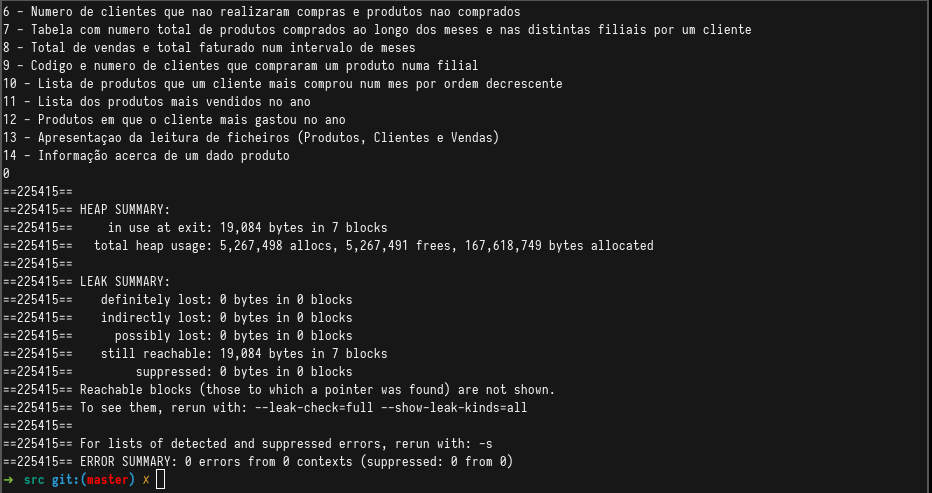
\includegraphics[width=\textwidth,height=4cm]{images/valgrind.png}
    \caption{Output do valgrind para uma execução do nosso programa}
\end{figure}

\newpage
\section{Conclusão}
Este projeto fez-nos principalmente questionar aquilo que sabemos sobre arquiteturas MVC e encapsulamento. Ao tomar a abordagem diferente que tomamos, aprendemos e questionamo-nos imenso acerca da natureza OO e o que motiva e torna tão simples utilizar esse paradigma para aplicações orientados ao utilizador em média-larga escala.

\vspace{0.5cm}
Foi também uma excelente oportunidade para melhorar os nossos conhecimentos sobre a linguagem de programação \textbf{C} e perceber que \textbf{Java} não se trata de nada mais que C com um \textit{garbage collector} e com alguma magia escondida. Achamos também interessante a possibilidade de alcançar features maioritariamente utilizadas no paradigma funcional como funções de ordem superior (a \textit{GLib} forçou-nos parte disso) para nos facilitar a vida no desenvolvimento de coisas monótonas e repetitivas, como é o caso do redirecionamento efetuado pelo menu principal.

\vspace{0.5cm}
\textbf{A nível de falhas do nosso projeto} achamos, sem dúvida, que o que nos podia trazer problemas a longo prazo caso o projeto continuasse a escalar é a nossa escolha de arquitetura. Obriga a codificar todas as ações de cada módulo no do SGV pelo que acabamos por ter alguma duplicação desnecessária. Note-se que a arquitetura é efetivamente funcional mas podia estar melhor. Parte da razão de não termos tentado trocar passa-se pelo facto de queremos aproveitar esta oportunidade para experimentar coisas diferentes e poder fazer algo muito sábio, aprender com os erros.

\vspace{0.5cm}
Em suma, este projeto permitiu-nos uma compreensão muito mais profunda de como os diferentes paradigmas se aproximam dos problemas e, além disso, permitiu-nos ver que, com algum esforço adicional, é possível aproximarmo-nos das vantagens de qualquer paradigma com o que quer que seja que estamos a trabalhar.

\end{document}
